\begin{figure}[tbh]
\centering
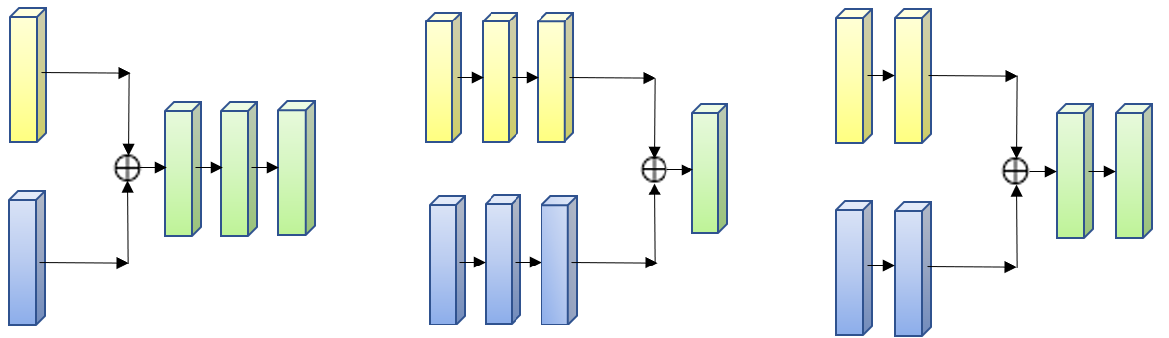
\includegraphics[width=\linewidth]{./images/early_late_middle_fusion.png}
\setlength{\abovecaptionskip}{-10pt plus 3pt minus 2pt}
\setlength{\belowcaptionskip}{-15pt plus 3pt minus 2pt}
\caption{Fusion schemes. Left: early fusion; Middle: late fusion; Right: middle fusion. Yellow and blue blocks symbolize features from distinct input branches, and green blocks represent fused data. Each block stands for a tensor of features. }
\label{fig:fusion}
\end{figure}